\chapter{Desserts}

\ChapterIntro{
    \lettrine{T}{his is the} chapter intro. \lipsum[1-3]
}

%
%
% Chocolate Chip Cookies
%
%
\newpage

\RecipeNameAndYield{Name=Chocolate Chip Cookies}

\RecipeStory{\lettrine{T}{stuff goes here} \lipsum[2]}

\begin{IngredientsAndSteps}
    \ListIngredientsAndSteps
    {
        2\fr1/2 cups all purpose flour

        1 teapoon baking soda

        \fr1/2 teapoon salt

        \IngredientsSeparatorClear

        1 cup butter, softened slightly

        \fr3/4 cup granulated sugar

        \fr3/4 cup packed light brown sugar

        \IngredientsSeparatorClear

        2 \tsp[s] vanilla

        2 large eggs

        12 \Ounce bag chocolate chips (2 cups)

        (optional) 1 cup chopped walnuts
    }
    {
        Preheat oven to 375\Degrees[F].

        Whisk the flour, baking soda, and salt in a small bowl.

        Cream the butter and sugars together until light and fluffy. You want to make sure you get
        enough air into the mixture and cut all that butter nicely.

        Add the vanilla and the eggs, one egg at a time. Beat the wet ingredients until quite smooth.

        Slowly add, about a cup at a time, the dry ingredients to the mixer and mix well.

        Once the dry and wet ingredients and combined beat on low-medium (3) until
        everything is smooth.

        Fold in the chocolate chips and, if using, the walnuts. Make sure they're well
        incorporated but do not over beat.

        Using a medium \#30 scoop spoon the dough onto parchment-lined cookie sheets.
    }
\end{IngredientsAndSteps}

\BakeUntil{Min=8, Max=10, GBrown=1}

\begin{ChefNotes}
    {If you make these with a \#20 scoop the recipe yields about 5 dozen cookies.}
\end{ChefNotes}

%
%
% Lemon Bars, Dad-style
%
%
\newpage

\RecipeNameAndYield{Name={Lemon Bars, Dad-style}}

% \begin{figure}
%     \centering
%     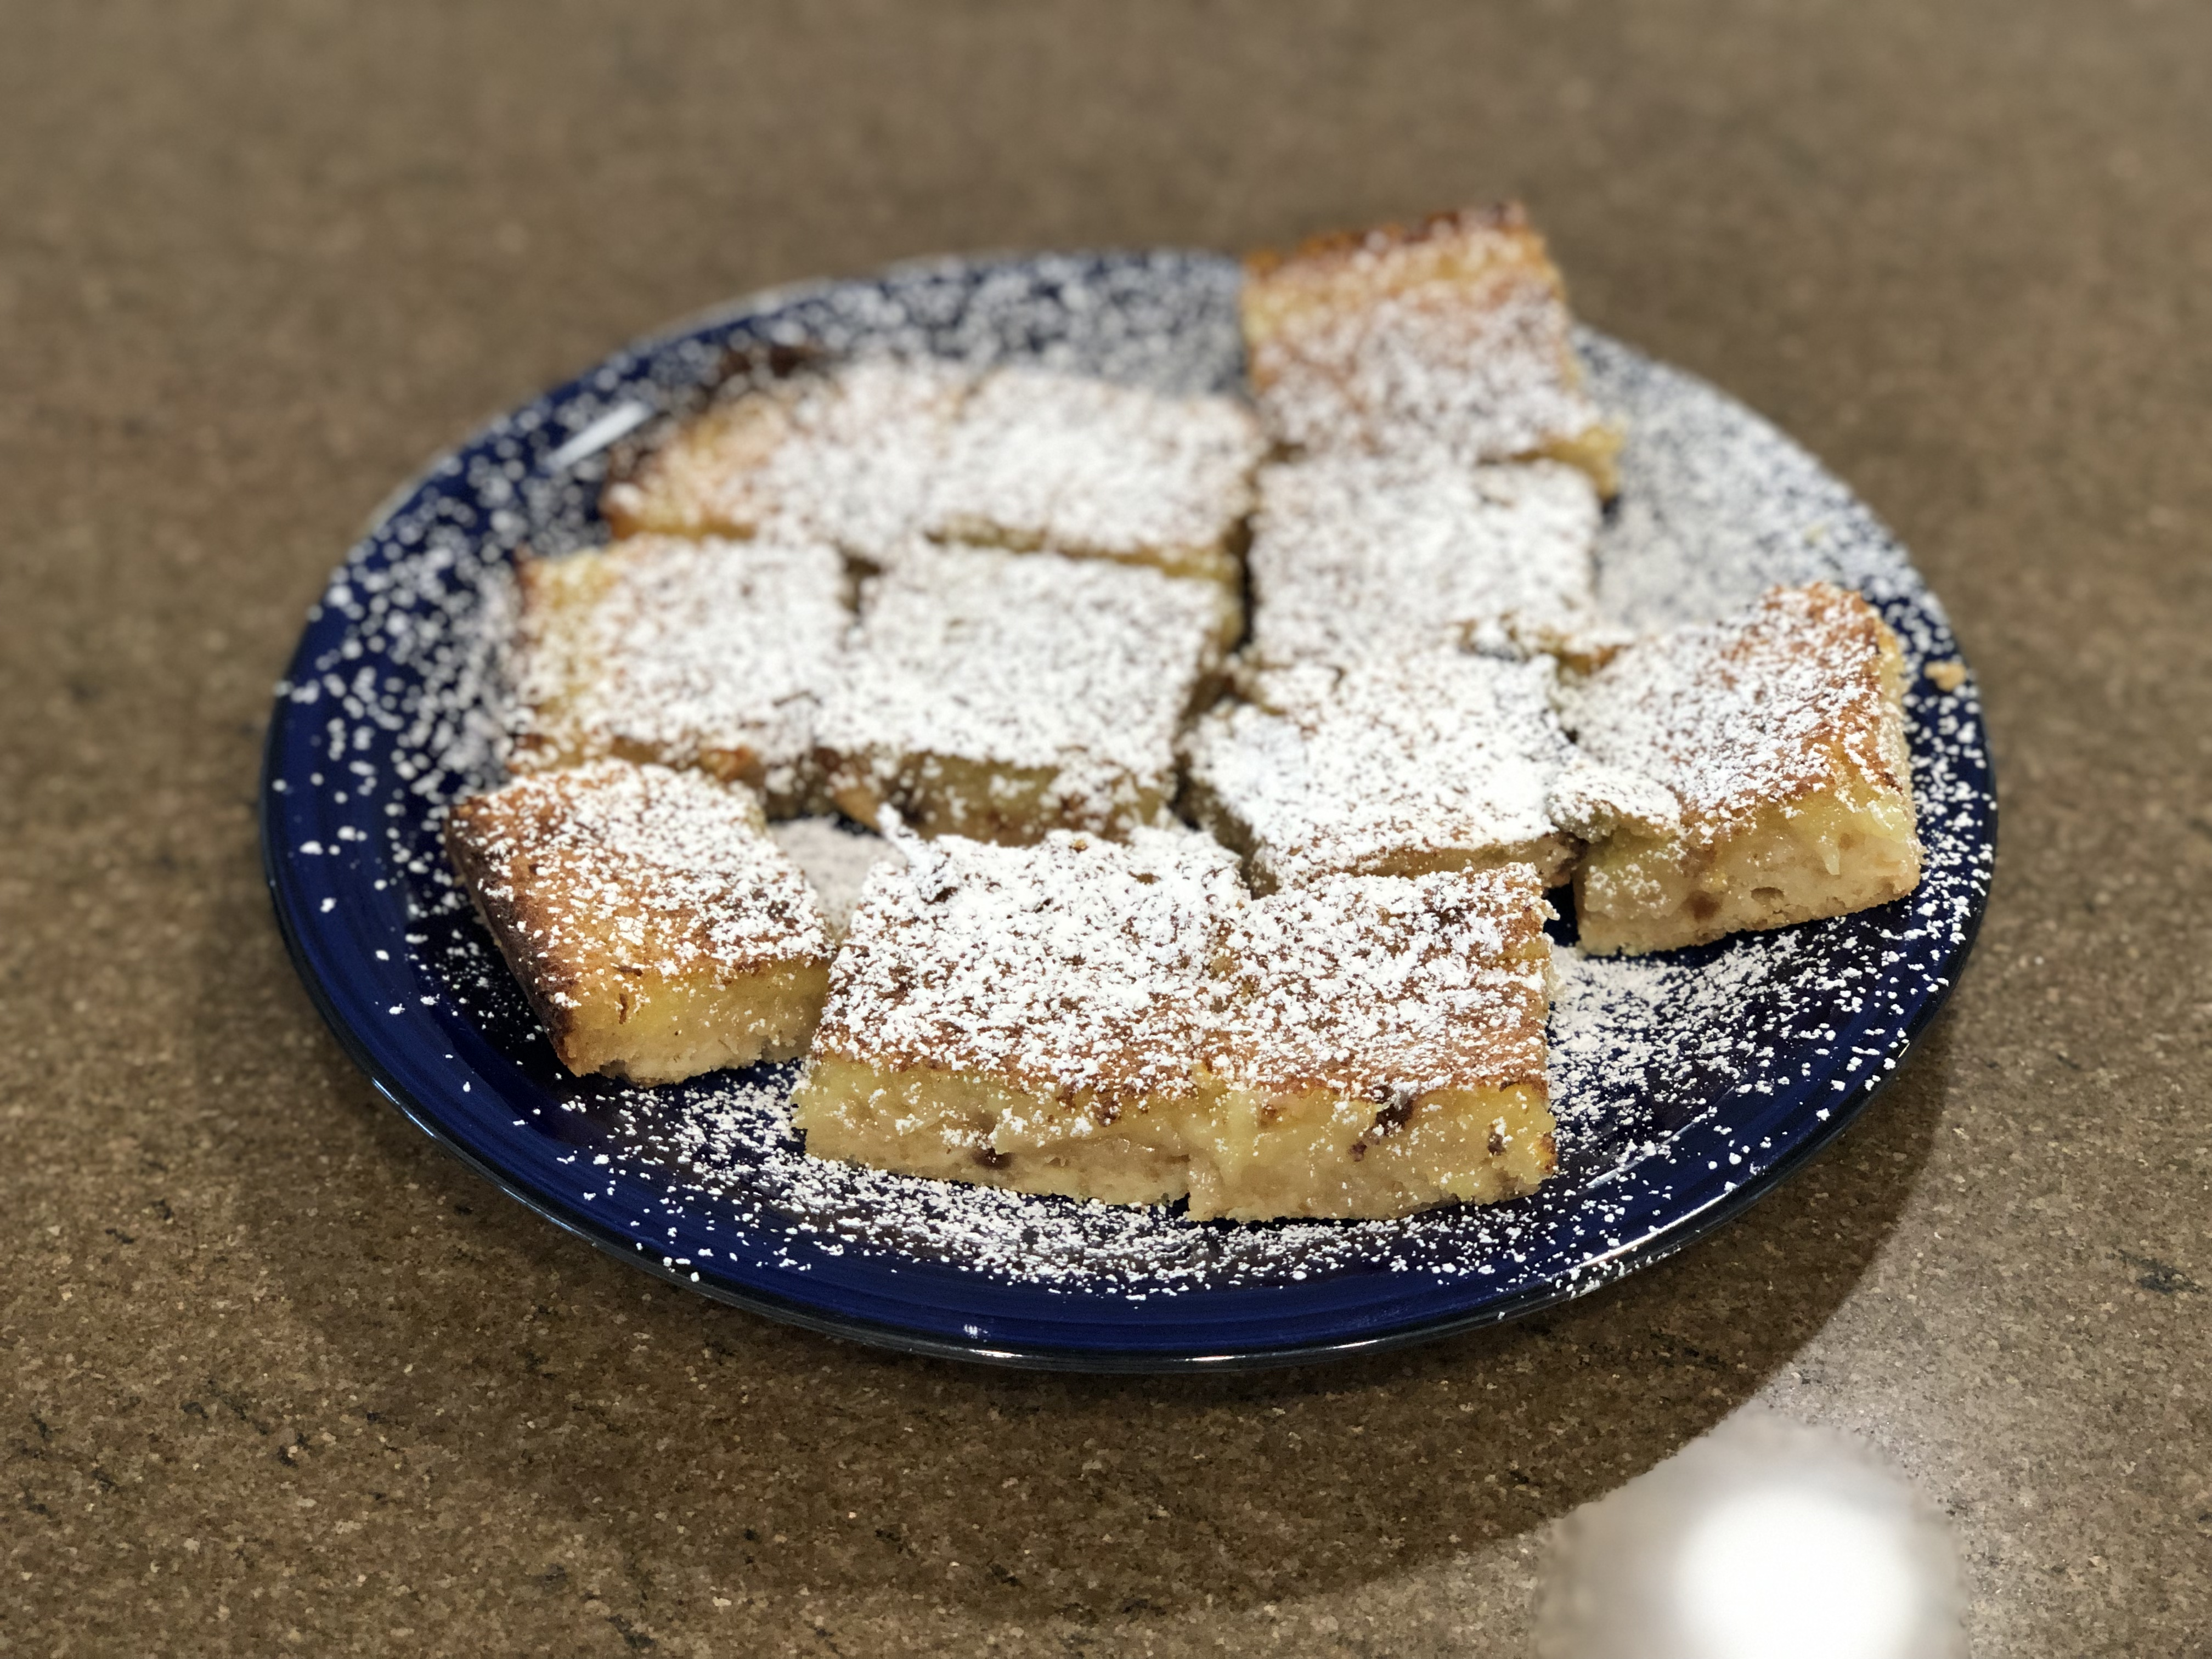
\includegraphics[scale=0.095]{lemon-bar.png}
% \end{figure}

\RecipeStory{\lettrine{T}{his is Pop Pop's favorite} sweet treat, and if there are fresh lemons from the tree out
    back then this is just something that you need to make. If you don't have your own
    lemon tree, well, store-bought lemons should be ok, but make sure they're really fresh.}

\begin{IngredientsAndSteps}
    \ListIngredientsAndSteps[Crust]
    {
        2 cups flour

        1 cup (2 sticks) butter, softened

        \fr1/2 cup powdered sugar

        \fr1/2 \tsp salt

        1 \Tbl light brown sugar

        1 \Tbl lemon zest
    }
    {
        Spray a \Inch{\AxB{9}{13}} glass baking dish with Pam and set aside.

        Mix the flour, powdered sugar, \fr1/2 \tsp salt, and light brown sugar
        with a whisk.

        Cut the butter into the flour if it's still cool. Or, if you've melted
        the butter, just stir it in. Stir in the 1 \Tbl lemon zest.

        Press this mixture into the bottom of the baking dish and bake at 350\Degrees[F] for 20 minutes.
    }

    \ListIngredientsAndSteps[Filling]
    {
        4 eggs, plus one egg yolk

        2 cups granulated sugar

        \fr1/4 \tsp salt

        2 - 3 \Tbl[s] lemon zest

        1 \tsp baking powder

        7 \Tbl[s] lemon juice
    }
    {
        While the crust is baking, combine the remaining ingredients in a medium bowl until
        well blended. You can use a whisk or an electric beater. Both work great.
    }

    \ListIngredientsAndSteps[Assembly]
    {
    }
    {
        When the crust finished immediately remove it from the oven and pour the egg mixture
        directly on top. Put this back in the 350 degree oven and bake for 15 to 20 minutes. Don't
        worry, it'll get brown spots on top in some spots. This is ok.

        Remove from oven and let the bars cool completely (yes Mom, completely). Then cut into
        \Inch{\AxB{2}{3}} pieces, move to a plate (this is the hard part, they're sticky), then dust
        with some more powdered sugar until they're white and pretty.
    }
\end{IngredientsAndSteps}

%
%
% M \& M Cookies
%
%
\newpage

\RecipeNameAndYield{Name=M \& M Cookies}

\RecipeStory{\lettrine{T}{his is a simple variation} on a classic Chocolate Chip Cookie recipe. I ended up making it one
    time when I only had a bag of mini M \& M's, didn't have the bag of chocolate chips, and was being
    asked (demanded of, actually) for some cookies.}

\begin{IngredientsAndSteps}
    \ListIngredientsAndSteps
    {
        2\fr1/2 cups all purpose flour

        1 teapoon baking soda

        \fr1/2 teapoon salt

        \IngredientsSeparatorClear

        1 cup butter, softened slightly

        \fr3/4 cup granulated sugar

        \fr3/4 cup packed light brown sugar

        \IngredientsSeparatorClear

        2 \tsp[s] vanilla

        2 large eggs

        12 \Ounce bag mini M \& M's (2 cups)
    }
    {
        Preheat oven to 375\Degrees[F].

        Whisk the flour, baking soda, and salt in a small bowl.

        Cream the butter and sugars together until light and fluffy. You want to make sure you get
        enough air into the mixture and cut all that butter nicely.

        Add the vanilla and the eggs, one egg at a time. Beat the wet ingredients until quite smooth.

        Slowly add, about a cup at a time, the dry ingredients to the mixer and mix well.

        Once the dry and wet ingredients and combined beat on low-medium (3) until
        everything is smooth.

        Fold in the M \& M's. Make sure they're well incorporated but do not over beat.

        Using a medium \#30 scoop spoon the dough onto parchment-lined cookie sheets.
    }
\end{IngredientsAndSteps}

\BakeUntil{Min=8, Max=10, GBrown=1}

\begin{ChefNotes}
    {If you make these with a \#20 scoop the recipe yields about 5 dozen cookies.}
\end{ChefNotes}

%
%
% Molasses Cookies
%
%
\newpage

\RecipeNameAndYield{Name=Molasses Cookies}

\RecipeStory{\lettrine{O}{k, this is one of those recipes} that started out somewhere else, and
    over time, has been changed enough to be considered mine now. Just in
    case you're wondering, this is also one of those recipes that converts
    peopleinto molasses cookie fans. Even the ones who say they don't like
    molasses cookies. Just sayin.

    Makes 22 cookies. Yeah, don't ask. That's how many it makes. So, I almost
    always double this recipe.

    For the best flavor, make sure that your spices are fresh. Light or mild
    molasses gives the cookies a milder flavor; for a stronger flavor, use
    dark or blackstrap molasses (this is what I use). Either way, measure
    the molasses in a liquid measuring cup. You can use the five spices to
    tune this recipe to your personal taste. I tend to make the first four
    ``heaping'' sized, but keep the black pepper right around \fr1/4 \tsp.
}

\begin{IngredientsAndSteps}
    \ListIngredientsAndSteps
    {
        2\fr1/4 cups (11\fr1/4 \Ounce[s]) all purpose flour

        1 \tsp baking soda

        2 \tsp[s] ground cinnamon

        2 \tsp[s] ground ginger

        \fr1/2 to \fr3/4 \tsp ground cloves

        \fr1/4 to \fr1/2 teapoon ground allspice

        \fr1/4 \tsp black pepper

        \fr1/4 \tsp salt

        \IngredientsSeparatorClear

        12 \Tbl[s] (1\fr1/2 sticks) unsalted butter softened but still cool

        \fr1/3 cup packed (2\fr1/3 \Ounce[s]) dark brown sugar

        \fr1/3 cup (2\fr1/3 \Ounce[s]) granulated sugar

        \fr1/2 cup raw sugar (for rolling)

        1 large egg yolk

        1 \tsp vanilla

        \fr1/2 cup light or dark molasses (see the note above)

    }
    {
        Adjust an over rack to the middle position and heat the oven to 375\Degrees[F]. Line a large baking sheet
        with parchment paper.

        Whisk the flour, baking soda, spices, and salt in a medium bowl and set aside.

        Cut the butter into \Tbl-sized pieces and beat on medium with the sugars until light and fluffy
        (about three minutes).

        Reduce speed to medium-low and add the egg yolk and vanilla; increase the speed to medium and beat
        until incorporated (about 30 seconds). Be sure to scrape the sides of the bowl at least once. Reduce
        speed to medium-low and add the molasses; beat until fully incorporated (about 30 seconds). Scrape the
        bottom and sides of the bowl at least once to avoid globs of butter. Reduce speed to lowest setting
        and add the flour mixture and beat until just incorporated. Once more with the scraping. This will
        take about 30 to 45 seconds.

        Use a \#30 cookie dough scoop to form balls and roll them in the raw sugar.
        Place 2 inches apart on the parchment-line baking sheets and bake for 10 minutes. The cookies will
        still look slightly undercooked. That's Ok. Don't try to bake two sheets at the same time unless
        you really trust your oven.

        Cool the cookies for 5 minutes on the baking sheet then move to a wire rack. Avoid the rush of people.
    }
\end{IngredientsAndSteps}

%
%
% Oatmeal Cookies
%
%
\newpage

\RecipeNameAndYield{Name=Oatmeal Cookies, Yield=About 30 cookies}

% \begin{figure}
%     \centering
%     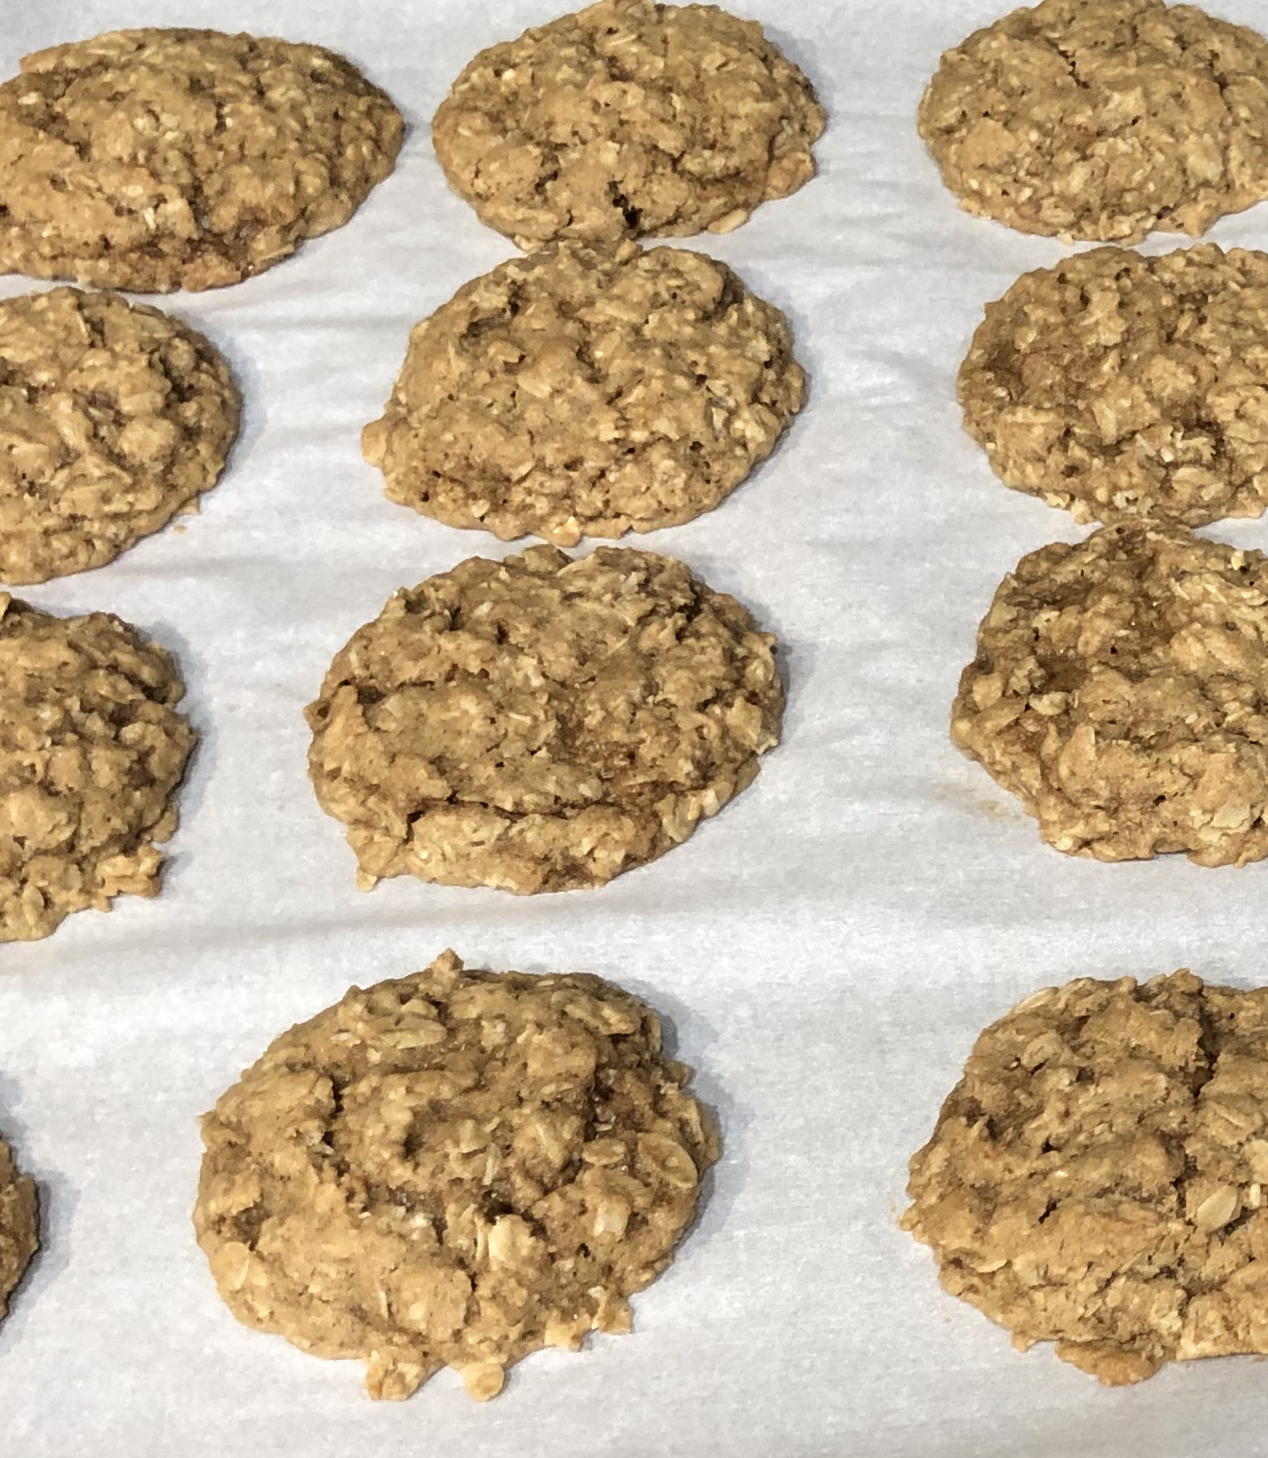
\includegraphics[width=0.5\textwidth]{oatmeal-cookies.png}
% \end{figure}

\RecipeStory{\lettrine{I} {started with the ``classic'' recipe} from the top of the Quaker Oats box. You know,
    the one that \emph{everyone} uses? Well, I was never really a fan because those
    cookies always came out flat and boring. Sometimes they'd be so flat it was like
    eating a very flat thing. Anyway, after a lot of experimentation (well, three or
    four batches), I came up with this recipe instead.}

\begin{IngredientsAndSteps}
    \ListIngredientsAndSteps
    {
        \fr1/2 cup (1 stick) plus 6 \Tbl[s] butter, cold

        \fr3/4 cup packed dark brown sugar

        \fr1/2 cup granulated sugar

        2 large eggs

        1\fr1/2 \tsp[s] vanilla

        1\fr3/4 cups, plus 2 \Tbl[s] flour

        1 \tsp baking soda

        2 \tsp[s] ground cinnamon

        \fr1/2 \tsp salt

        3\fr1/4 cups Quaker Oats

        (optional) 1 cup craisins or raisins
    }
    {
        Adjust an over rack to the middle position and heat the oven to 350\Degrees[F]. Line a large baking sheet
        with parchment paper.

        Whisk the flour, baking soda, cinnamon, oats, and salt in a medium bowl and set aside.

        Cut the butter into \Tbl-sized pieces and beat on medium with the sugars until light and fluffy
        (about three minutes).

        Reduce speed to medium and add the eggs and vanilla. Increase speed to medium-high and beat until
        light and fluffy (the mixture will appear to double in size).

        Add the dry ingredients one cup at a time until fully incorporated. Scrap the sides of the
        bowl and mix at least one more time.

        Use a \#30 cookie dough scoop (the medium one) to form balls of dough.
        Place 2 inches apart on the parchment-lined baking sheets and bake for 9 minutes until just starting
        to turn medium brown. The cookies will still look slightly undercooked.

        Cool the cookies for 5 minutes on the baking sheet then move to a wire rack. Avoid the rush of people.
    }
\end{IngredientsAndSteps}

\begin{Tip}
    {After making these Bill, Min's dad, mentioned that he'd made oatmeal cookies in the past using
        Grand Marnier. That made me wonder if adding some grated orange peel would be good. Turns out that
        I had one of these that happened to be sitting very close to a Sumo orange and the flavor
        combination was \emph{nice}. So, I'm tempted to do this in my next batch.}
\end{Tip}

%
%
% Peanut Butter Thumbprints
%
%
\newpage

\RecipeNameAndYield{Name=Peanut Butter Thumbprints}

\RecipeStory{\lettrine{T}{stuff goes here} \lipsum[2]}

\begin{IngredientsAndSteps}
    \ListIngredientsAndSteps
    {
        48 Hershey Kisses, unwrapped

        \IngredientsSeparatorClear

        \fr1/2 cup shortening

        \fr3/4 cup chunky peanut butter

        \fr1/3 cup granulated sugar

        \fr1/3 packed light brown sugar

        \IngredientsSeparatorClear

        1 egg

        2 \Tbl[s] milk

        2 \tsp[s] vanilla

        \IngredientsSeparatorClear

        1\fr1/2 cups all purpose flour

        1 teapoon baking soda

        \fr1/2 teapoon salt

        \fr1/2 cup granulated sugar for rolling
    }
    {
        Preheat oven to 375\Degrees[F].

        Beat hard the shortening and peanut butter with the granulated and brown sugars
        until light and fluffy, about 3 minutes. Make sure to scrape the sides of the
        mixer several times.

        On medium speed beat in the egg, milk, and vanilla.

        Whisk the flour, baking soda, and salt in a medium bowl. Gradually mix the dry ingredients
        into the peanut butter mixture.

        Using the medium scoop form balls of dough. Roll each each ball in a bowl with the
        additional granulated sugar.

        Place the balls on a parchment lined cookie sheet. You should put about 12 cookies
        on each sheet.

        Bake 8 to 10 minutes or until lightly browned. Immediately press a kiss into the center
        of each cookie (they're going to crack around the edges, this is ok).

        Slide the cookies and parchment to a wire cooling rack and cool completely.
    }
\end{IngredientsAndSteps}

%
%
% peanut-butter
%
%
\newpage

\RecipeNameAndYield{Name=Peanut Butter}

\RecipeStory{\lettrine{I}{t's always fun to smash} up ingredients. It really is. In this case we get to smash up some peanuts to
    make a really chunky version of our own peanut butter. Don't worry, we're going to add even more
    chunky peanut butter while we're going. These peanut butter cookies end up with a nice smooth texture
    because there's so much butter. If you don't like ``sandy'' peanut butter cookies then these are for you.

    These cookies, if done right, end up thick and chewy with just the right amount of slightly sweet-salty
    peanutty flavor. Oh, the honey, that's because honey is hygroscopic, which means it attracts water
    and helps keep the cookies moist. After you unwrap the butter keep the wrappers as they'll have just
    enough butter left to coat the bottom of the glass.}

\begin{IngredientsAndSteps}
    \ListIngredientsAndSteps
    {
        2\fr1/2 cups all purpose flour

        \fr1/2 teapoon baking powder

        \fr1/2 teapoon baking soda

        \fr1/4 teapoon salt

        \IngredientsSeparatorClear

        \fr3/4 cup butter

        \fr1/3 cup granulated sugar

        1 cup packed light brown sugar

        \fr3/4 cup chunky peanut butter

        1 \Tbl honey

        1 \tsp vanilla

        2 large eggs

        \IngredientsSeparatorClear

        1\fr1/2 cups salted snacking peanuts

        granulated sugar for sprinkling
    }
    {
        Preheat oven to 375\Degrees[F].

        Mix the flour, baking powder, baking soda, and salt in a small bowl.

        Cream the butter and sugars together until light and fluffy. You want to make sure you get
        enough air into the mixture and cut all that butter nicely.

        Add the peanut butter, honey, eggs, and vanilla and beat until light and fluffy again.

        Put the peanuts in a zipper lock bag and roll them until they are like a coarse sand. You
        don't want mush, but you don't want whole peanuts either.

        Using a medium \#30 scoop spoon the dough onto parchment-lined cookie sheets. Using
        the bottom of a buttered and sugared glass press the cookies until they are between \fr1/2
        and \fr3/4 inches thick. Make sure you're consistent. Sprinkle each cookie with a little
        more granulated sugar.

        Bake for 9 to 10 minutes or until done, but do not overbake them. Let them sit on the baking
        sheet for a few additional minutes before removing to a wire rack to completely cool.
    }
\end{IngredientsAndSteps}

%
%
% Snickerdoodles
%
%
\newpage

\RecipeNameAndYield{Name=Snickerdoodles}

% \begin{figure}
%     \centering
%     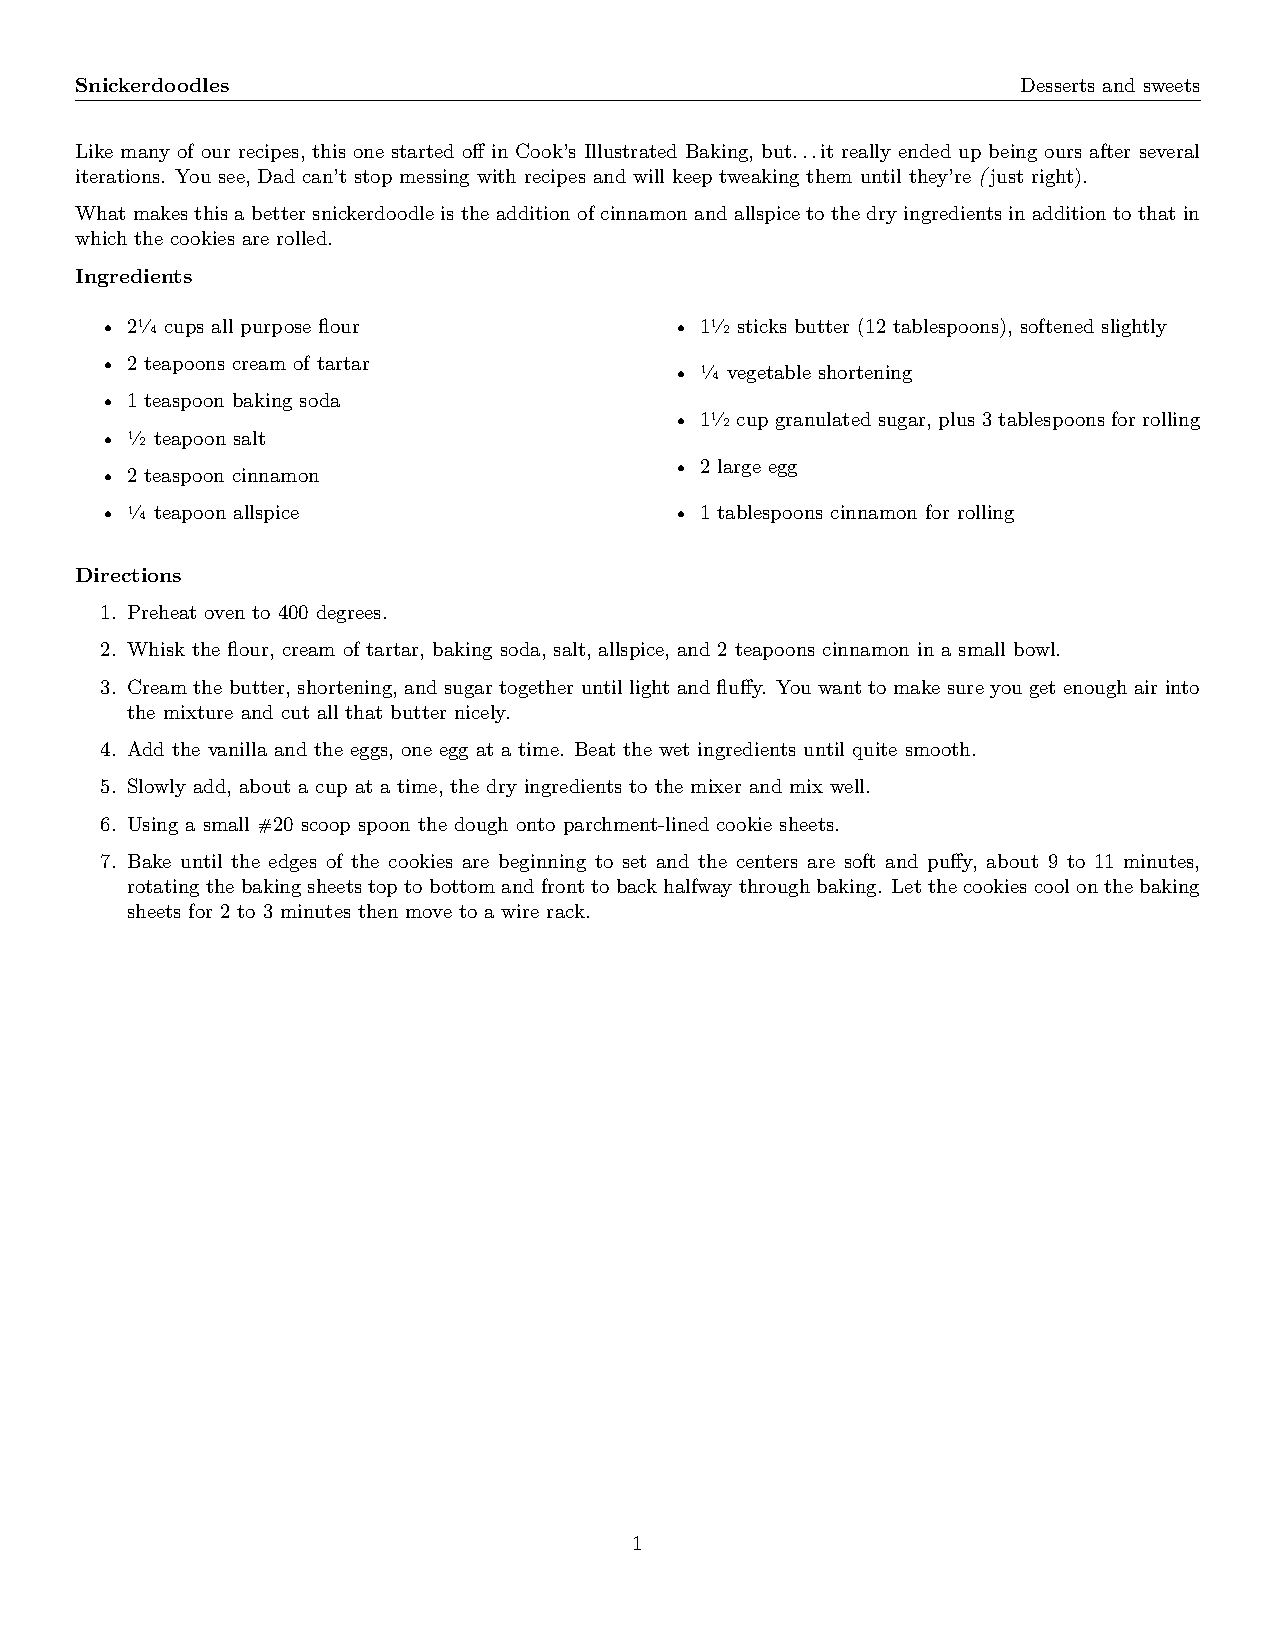
\includegraphics[scale=0.025]{snickerdoodles.png}
% \end{figure}

\RecipeStory{\lettrine{L}{ike many of our recipes}, this one started off in Cook's Illustrated Baking, but\dots it really
    ended up being ours after several iterations. You see, Dad can't stop messing with recipes and will
    keep tweaking them until they're \textit{just right}.

    What makes this a better snickerdoodle is the addition of cinnamon and allspice to the
    dry ingredients in addition to that in which the cookies are rolled.}

\begin{IngredientsAndSteps}
    \ListIngredientsAndSteps
    {
        2\fr1/2 cups all purpose flour

        2 teapoons cream of tartar

        1 \tsp baking soda

        \fr1/2 teapoon salt

        2 \tsp[s] cinnamon

        \fr1/4 teapoon allspice

        \IngredientsSeparatorClear

        1\fr1/2 sticks butter (12 \Tbl[s]), at room temperature

        \fr1/4 cup vegetable shortening, at room temperature

        1\fr1/2 cups granulated sugar, plus 3 \Tbl[s] for rolling

        2 large eggs, at room temperature

        1 \Tbl cinnamon plus \fr1/3 cup granulated sugar for rolling

    }
    {
        Preheat oven to 400\Degrees[F].

        Whisk the flour, cream of tartar, baking soda, salt, allspice, and the 2 teapoons cinnamon
        in a small bowl.

        Mix the butter, shortening, and sugar together until just combined. DO NOT overmix. Run at
        medium speed, for about 1\fr1/2 minutes.

        Add the eggs and blend until just combined.

        Add the dry ingredients to the mixer and mix until dough is smooth.

        Using a small \#20 scoop, drop the dough into the sugar and cinnamon mixture and
        evenly coat.

        Put the dough rounds on a jelly roll pan and chill at least one hour.

        Bake until the edges of the cookies are beginning to set and the centers are soft
        and puffy, about 9 minutes. Let the cookies cool on the baking sheets for 2 to 3
        minutes then move to a wire rack. The cookies might appear slightly under done. This
        is expected and ok.
    }
\end{IngredientsAndSteps}

%
%
% Sugar Cookies
%
%
\newpage

\RecipeNameAndYield{Name=Sugar Cookies}

\RecipeStory{\lettrine{Y}{et another Cooks Illustrated} Baking-inspired recipe. But, as with most of the recipes in that
    book, Dad had to mess with it\dots

    These are not decoration sugar cookies. That's a completely different recipe. These are soft
    and chewy.}

\begin{IngredientsAndSteps}
    \ListIngredientsAndSteps
    {
        2\fr1/4 cups all purpose flour

        \fr1/2 teapoon baking powder

        \fr1/4 teapoon salt

        \IngredientsSeparatorClear

        2 sticks butter, softened slightly, but still cool

        1 cup granulated sugar, plus \fr1/2 for rolling

        1 \Tbl light brown sugar

        \IngredientsSeparatorClear

        1 large egg

        2 \tsp[s] vanilla
    }
    {
        Preheat oven to 375\Degrees[F].

        Whisk the flour, baking powder, and salt in a small bowl.

        Cream the butter and sugars together until light and fluffy. You want to make sure you get
        enough air into the mixture and cut all that butter nicely.

        Add the vanilla and the eggs, one egg at a time. Beat the wet ingredients until quite smooth.

        Add the dry ingredients to the mixer and mix well.

        Using a medium \#30 scoop spoon the dough onto parchment-lined cookie sheets.

        Roll each dough ball in the granulated sugar until well coated.

        Using the bottom of a flat-bottomed glass, coated in butter and dipped in sugar,
        flatten the cookied to \fr3/4 inch thick

        Bake for 15 to 18 minutes rotating the pans top to bottom and back to front halfway
        through baking. Let cool 3 minutes on the baking sheet before moving to a wire rack.
    }
\end{IngredientsAndSteps}

\begin{ChefNotes}
    {I just happened to have picked a bunch of fresh lemons one morning when I
        made these. So, I made a quick lemon glaze using about \fr1/2 cup powdered sugar and
        just enough lemon juice to make a spreadable glaze. After the cookies are completely cooled,
        pour the glaze over them.

        Another alternative, since these are really light cookies is to grate 2 to 3 \Tbl[s] of
        lemon zest into the wet ingredients to create a simple lemon sugar cookie. If you do this you
        might want to cut the vanilla in half to 1 teapoon, increase the flour \fr1/4 cup and
        add 2 teapoons of lemon juice.}
\end{ChefNotes}
%
%
% Todd Bardal Cookies
%
%
\newpage

\RecipeNameAndYield{Name=Todd Bardal Cookies}

\RecipeStory{\lettrine{T}{his recipe came from Nana's} ``black book'' of recipes. We don't know where she got it, probably
    from the NY Times. We've been making these \textit{forever} now and they're always a hit.}

\begin{IngredientsAndSteps}
    \ListIngredientsAndSteps
    {
        1\fr3/4 cups all purpose flour

        \fr1/2 teapoon baking soda

        \fr1/2 teapoon salt

        \IngredientsSeparatorClear

        \fr1/2 cup butter, softened slightly

        \fr1/2 cup granulated sugar

        \fr1/2 cup packed light brown sugar

        \IngredientsSeparatorClear

        1 \tsp vanilla

        1 large egg

        \fr1/4 cup peanut butter

        1 cup chocolate chips (\fr1/2 package)
    }
    {
        Preheat oven to 375\Degrees[F].

        Whisk the flour, baking soda, and salt in a small bowl.

        Cream the butter and sugars together until light and fluffy. You want to make sure you get
        enough air into the mixture and cut all that butter nicely.

        Add the vanilla and the eggs, one egg at a time. Beat the wet ingredients until quite smooth.

        Slowly add, about a cup at a time, the dry ingredients to the mixer and mix well.

        Fold in the chocolate chips and, if using, the walnuts. Make sure they're well
        incorporated but do not over beat.

        Using a medium \#30 scoop spoon the dough onto parchment-lined cookie sheets.

        Bake for 10 to 12 minutes or until done or until just starting to turn golden brown.
    }
\end{IngredientsAndSteps}

%
%
% White Chocolate Macadamia Cookies
%
%
\newpage

\RecipeNameAndYield{Name=White Chocolate Macadamia Cookies}

\RecipeStory{\lettrine{T}{his recipe makes a bunch} of cookies. How many? Well, about 6 dozen. Doesn't seem possible does it? Well,
    if you follow the directions and use a \#20 scoop you'll end up with that many tasty bite-sized
    cookies. You can also use a \#30 scoop to get slightly larger cookies. Buyer beware though because
    these are really rich.}

\begin{IngredientsAndSteps}
    \ListIngredientsAndSteps
    {
        3 cups all purpose flour

        \fr1/2 teapoon baking soda

        1 teapoon salt

        1 cup butter, softened slightly

        1\fr1/2 cups granulated sugar

        \fr1/2 cup packed light brown sugar

        2 large eggs

        1\fr1/2 \tsp vanilla

        12 \Ounce bag white chocolate chips (2 cups)

        1\fr1/2 cups coarsely chopped macadamia nuts
    }
    {
        Preheat oven to 350\Degrees[F].

        Whisk the flour, baking soda, and salt in a small bowl.

        Cream the butter and sugars together until light and fluffy. You want to make sure you get
        enough air into the mixture and cut all that butter nicely.

        Add the vanilla and the eggs, one egg at a time. Beat the wet ingredients until quite smooth.

        Slowly add, about a cup at a time, the dry ingredients to the mixer and mix well.

        Once the dry and wet ingredients and combined beat on low-medium (3) until
        everything is smooth.

        Fold in the white chocolate chips and the macadamia nuts. Make sure they're well
        incorporated but do not over beat.

        Using a small \#20 scoop spoon the dough onto parchment-lined cookie sheets.

        Bake for 10 to 12 minutes or until done or until just starting to turn golden brown.
    }
\end{IngredientsAndSteps}

\begin{ChefNotes}
    {Do not overbake these as they'll get quite dry and crunchy quickly. I tend to pull
        them a minute or so early (at 11 minutes) and let them finish on the baking sheet out of the oven.
        This leaves the cookies nice and soft in the middle with just enough crunch around the edges.}
\end{ChefNotes}
